\question[5] Un tigre camina hacia adelante y hacia atrás a lo largo de un borde rocoso. Su movimiento se muestra en la siguiente gráfica (Fig. \ref{fig:dist_tiempo_04}) de la posición vertical,
$y$, en funci\'on del tiempo, $t$. \par

{\InsertBoxR{0}{
    \parbox[t]{0.5\linewidth}{
        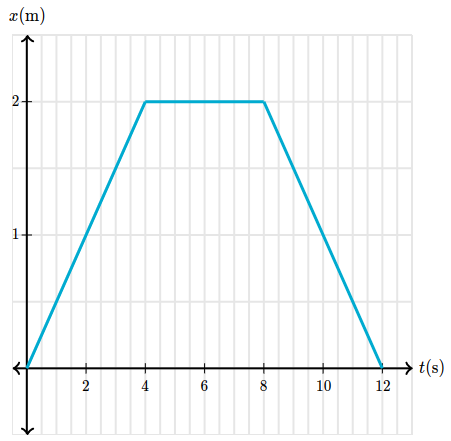
\includegraphics[width=\linewidth]{Images/dist_tiempo_04}
        \label{fig:dist_tiempo_04}
        \captionof{figure}{La gráfica representa el movimiento del tigre.}%
    }
}}
\hspace{0.5cm}
\begin{minipage}[t]{0.4\linewidth}
    \begin{parts}
        %  \begin{minipage}[t]{0.45\linewidth}
        \subfile{Questions/Parts/question008a}
        \subfile{Questions/Parts/question008b}
        %   \end{minipage}%
        % \subfile{Questions/Parts/question008c}
        % \subfile{Questions/Parts/question008d}
        \subfile{Questions/Parts/question008e}
        \subfile{Questions/Parts/question008f}
        % \subfile{Questions/Parts/question008g}
        % \subfile{Questions/Parts/question008h}
    \end{parts}
\end{minipage}